\subsection{The Ball and the Boat Problem}

This is a classic problem, but I first did a proper analysis of it when I was looking for Oxbridge mock interview questions and my friend, Dami from WSP, suggested it. This requires only very basic understanding of physics and does not need any particular tricks or special insights to solve, but is nevertheless quite pleasing. I rate this problem a 2 out of 10 in terms of difficulty.

Suppose there is a small boat in a pool with a person and a ball onboard. The person throws the ball overboard. What happens to the water level in the following cases?

\begin{enumerate}
    \item The ball sinks to the bottom.
    \item The ball floats on the surface.
    \item The ball floats but it is then tied to the bottom of the pool.
    \item The ball floats but the person in the boat forces it underwater so it is fully submerged.
\end{enumerate}

\textbf{Hints:}

\begin{enumerate}
    \item Remember Archimedes' principle - the buoyant force acting on an object is equal to the weight of fluid it displaces, and acts in the upwards direction.
    \item Consider extreme cases - a very dense ball and a ball with very low density.
    \item Identify the different systems and the forces acting on them.
\end{enumerate}

\textbf{Solution:}

The key to this problem is understanding difference between buoyant forces caused by the mass of the ball and the volume of the ball. When the ball is in the boat, the buoyant force is due to the weight of the ball and is independent of the volume. When the ball is in the water, the buoyant force is due to the volume of the ball and is independent of the weight. The forces in the original situation are shown in figure~\ref{fig:TheBallAndTheBoat_Setup}, and the four cases are shown in figure~\ref{fig:TheBallAndTheBoat}.

When the ball is in the boat, the additional weight pushes the boat deeper into the water, meaning a greater volume of the boat is under the water line. This means a greater volume of water is displaced, and thus a greater weight of water is displaced, and therefore a larger buoyant force. This force is a function only of the weight of the ball as changing the volume of the ball only displaces air inside the boat. When the ball is fully submerged, the volume of water displaced is equal to the volume of the ball and therefore the weight of the ball is irrelevant. If the ball is floating, then by Archimedes' principle the weight of the water displaced by the volume of the ball is equal to the weight of the ball.

This understanding can be used to construct a force balance. When the ball is in the boat, the boat and the ball are treated together as a single system. The two forces are the weight of the ball and the boat combined acting downwards, and an equal and opposite buoyant force acting upwards. When the ball is fully submerged, the ball and the boat need to be treated as separate systems. As before, the boat has two forces acting on it, the weight of the boat and the equal and opposite buoyant force. The case for the ball is different however. The ball has a weight acting downwards, but now there are two forces acting upwards. The buoyant force is equal to the weight of water displaced by the ball and there is also a reaction force from the bottom of the pool stopping the ball falling through the floor.

In both cases, the systems are in equilibrium and the total downwards forces are equal, meaning the upwards forces must be equal in both cases as well. As there is a contact force when the ball is submerged, the total buoyant force must be less than when the ball is in the boat. The buoyant force is equal to the weight of the water displaced, and as the water is of constant density, this is proportional to the volume of water displaced. This means less water is displaced when the ball is submerged compared to being in the boat, and thus the water level is lower. We could also see this by noting the weight of the ball must be greater than the weight of the water it displaces because it is denser than water.

Similar reasoning can be applied in the other parts of the question. If the ball floats on the surface or has a density equal to that of water there is no contact force. The total system weight is equal to the total system buoyant force in both cases, meaning the water level stays the same. If the ball has a density less than water but is forced under the surface anyway, the buoyant force is more than the weight. Instead of a contact force acting upwards, a tension in the rope acts downwards to maintain equilibrium. The greater total buoyant force means more water is displaced, giving a higher water level.

The final part is almost identical to the second part. The total buoyant force is equal to the total weight as there are no other forces acting on the system and it is in equilibrium. As before this leads to the water lever staying the same. Understanding the individual forces on the ball and boat is still interesting however. The buoyant force on the ball is split into two parts, one equal to the weight of the ball, and the remaining buoyancy is additional buoyancy. As the weight of the boat is smaller than the boat and the ball combined, the boat will float higher in the water due to a smaller volume needing to be displaced. This loss in buoyancy is exactly equal to the additional buoyancy from the ball. Compared to the second part of the question, the boat sits higher in the water and the ball sits lower, with the total water displaced remaining exactly equal.

\textbf{Extensions and Comments:}

This is a problem where thinking of extreme cases helps elucidate the principles. Consider a very tiny ball of constant size and large mass. The difference in water level when the ball is in the water or completely removed from the system is negligible due to the small size of the ball. Increasing the weight makes no difference at all. If the ball was put into the boat however, the boat would sit much lower in the water. Increasing the weight of the ball would cause it to sit even lower, and clearly the volume of water displaced increases. A very light ball with a large varying volume demonstrates part three nicely. This makes very little difference to how deep the boat sits in the water, and is independent of the volume. When increasing the volume when it is submerged, the volume of water displaced increases, and the water level clearly increases.

\begin{figure}[H]
    \centering
    \begin{subfigure}{0.49\textwidth}
        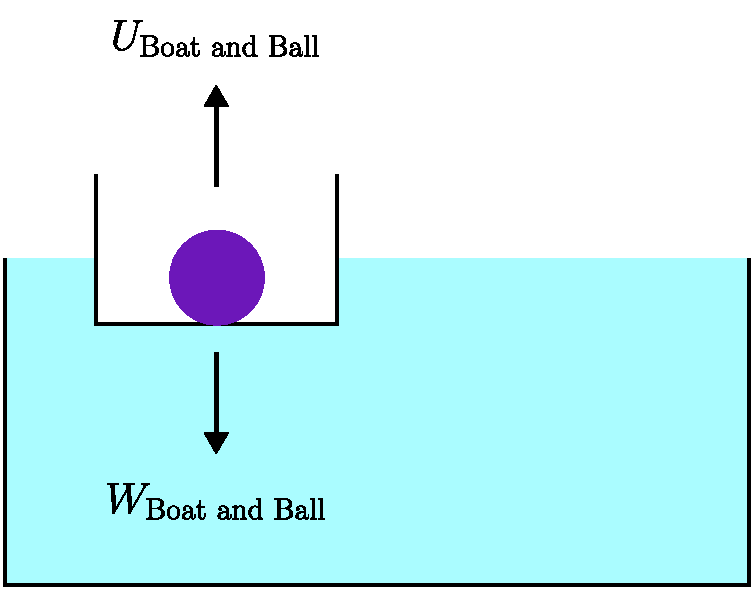
\includegraphics[width=\textwidth]{5 - Physics/TheBallAndTheBoat_Setup.pdf}
    \end{subfigure}
    \caption{The forces acting on the original system}
    \label{fig:TheBallAndTheBoat_Setup}
\end{figure}

\begin{figure}[H]
    \centering
    \begin{subfigure}{0.49\textwidth}
        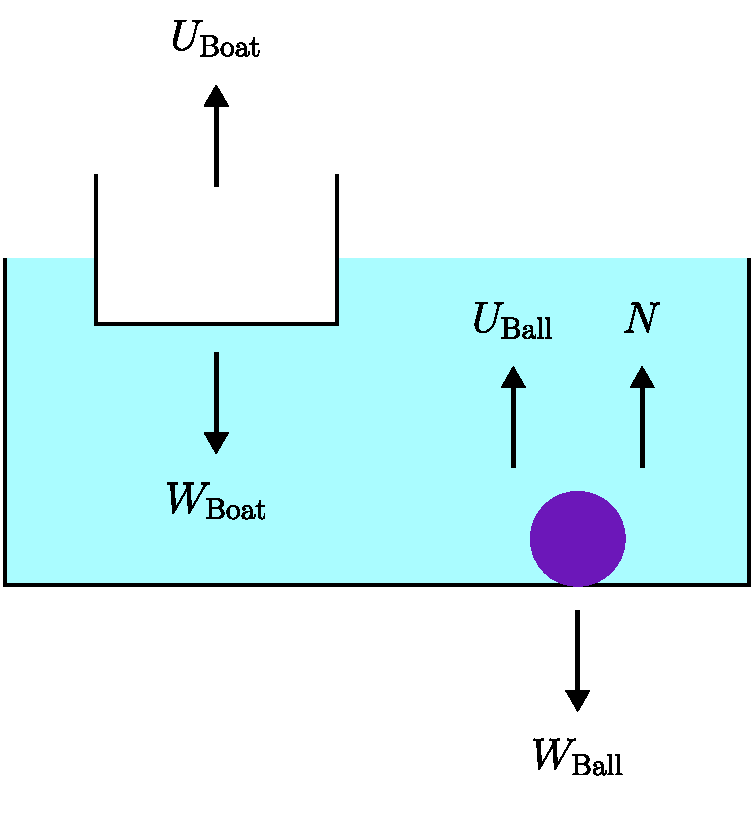
\includegraphics[width=\textwidth]{5 - Physics/TheBallAndTheBoat_Case1.pdf}
        \caption{Part 1}
        \label{fig:TheBallAndTheBoat_Case1}
    \end{subfigure}
    \hfill
    \begin{subfigure}{0.49\textwidth}
        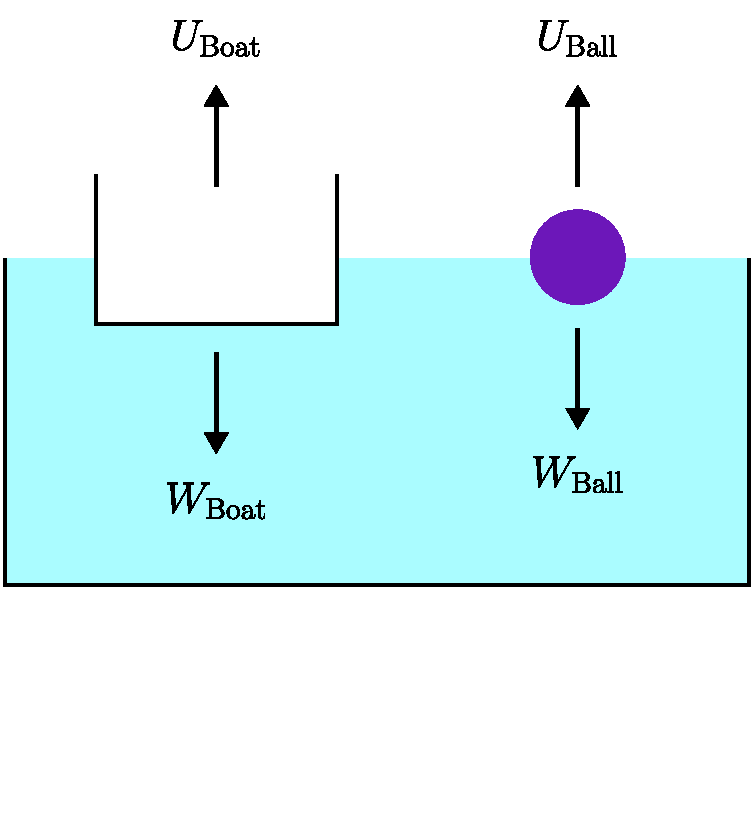
\includegraphics[width=\textwidth]{5 - Physics/TheBallAndTheBoat_Case2.pdf}
        \caption{Part 2}
        \label{fig:TheBallAndTheBoat_Case2}
    \end{subfigure}  \\
    \vspace{10mm}
    \begin{subfigure}{0.49\textwidth}
        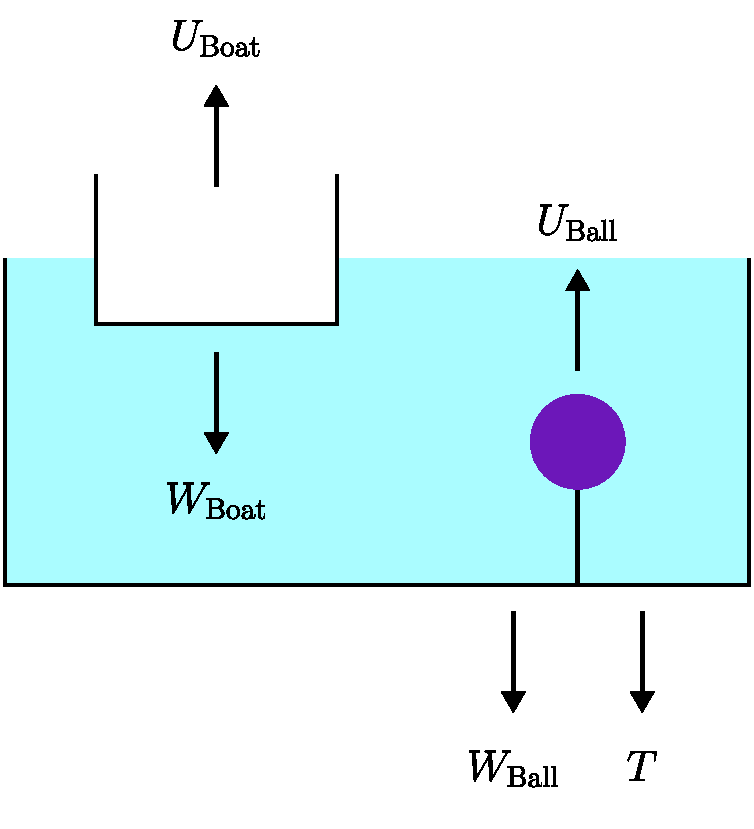
\includegraphics[width=\textwidth]{5 - Physics/TheBallAndTheBoat_Case3.pdf}
        \caption{Part 3}
        \label{fig:TheBallAndTheBoat_Case3}
    \end{subfigure}
    \hfill
    \begin{subfigure}{0.49\textwidth}
        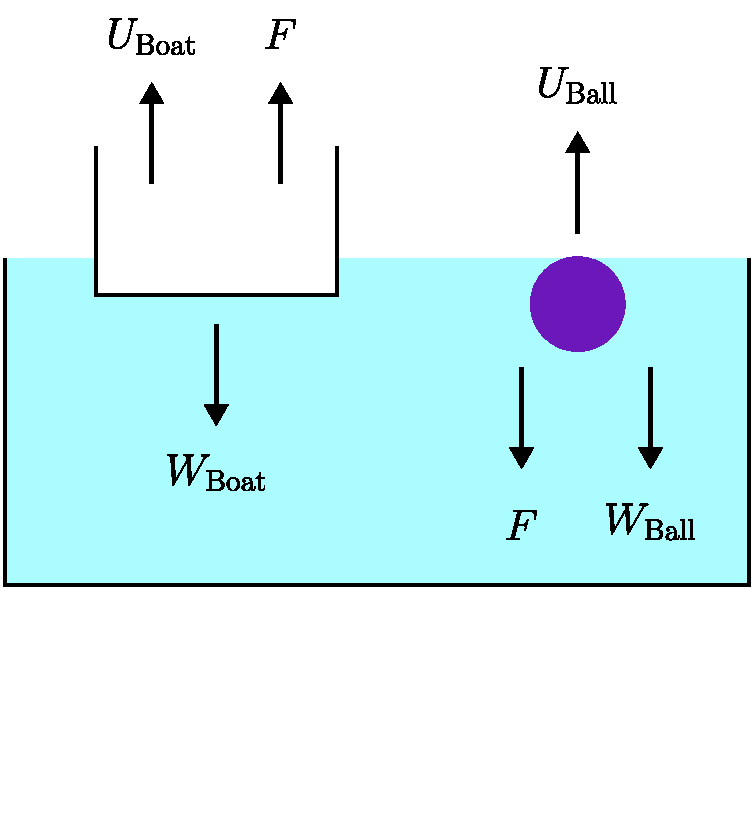
\includegraphics[width=\textwidth]{5 - Physics/TheBallAndTheBoat_Case4.pdf}
        \caption{Part 4}
        \label{fig:TheBallAndTheBoat_Case4}
    \end{subfigure}
    \caption{The forces acting on the ball and the boat in each of the four parts}
    \label{fig:TheBallAndTheBoat}
\end{figure}